

                           
\documentclass[12pt,twoside]{article}

%%%%%%%%%%%%%%%%
% Adding the include only list allows you to typeset only your
% chapter while maintaining overall page numbers and references.
% It also shields you from errors in other chapters as you go along.
% You need to typeset the whole thing once though. 

%\includeonly{title_page,daq_trig/daq_trig}

%%%%%%%%%%%%%%%%%%  header  (packages, 
\input{header}

\begin{document}
\linenumbers
%\frontmatter
\pagestyle{empty}

%%%%%%%%%%%%%%%%%%%%%%%%%%%%%%%%% title page
\renewcommand*\familydefault{\sfdefault}
{\sffamily
\vfill
\vspace{4cm}
\begin{figure}[H]
  \begin{center}
  \includegraphics[width=0.3\linewidth]{figs/ecce-logo.png}
\end{center}
\end{figure}

\begin{center}
  \large
  {\LARGE{ECCE Note 2021-01}}

  \begin{tabular}{cc}
&Notes on Re-Use of the BaBar Solenoid in ECCE \\
&P. Brindza, D. Higinbotham, J. Lajoie, \\
&R. Rajput-Ghoshal, S. Tapia \\
&\today
\\
  \end{tabular}
  \end{center}

\vspace{1cm}

\begin{figure}[H]
  \begin{center}
    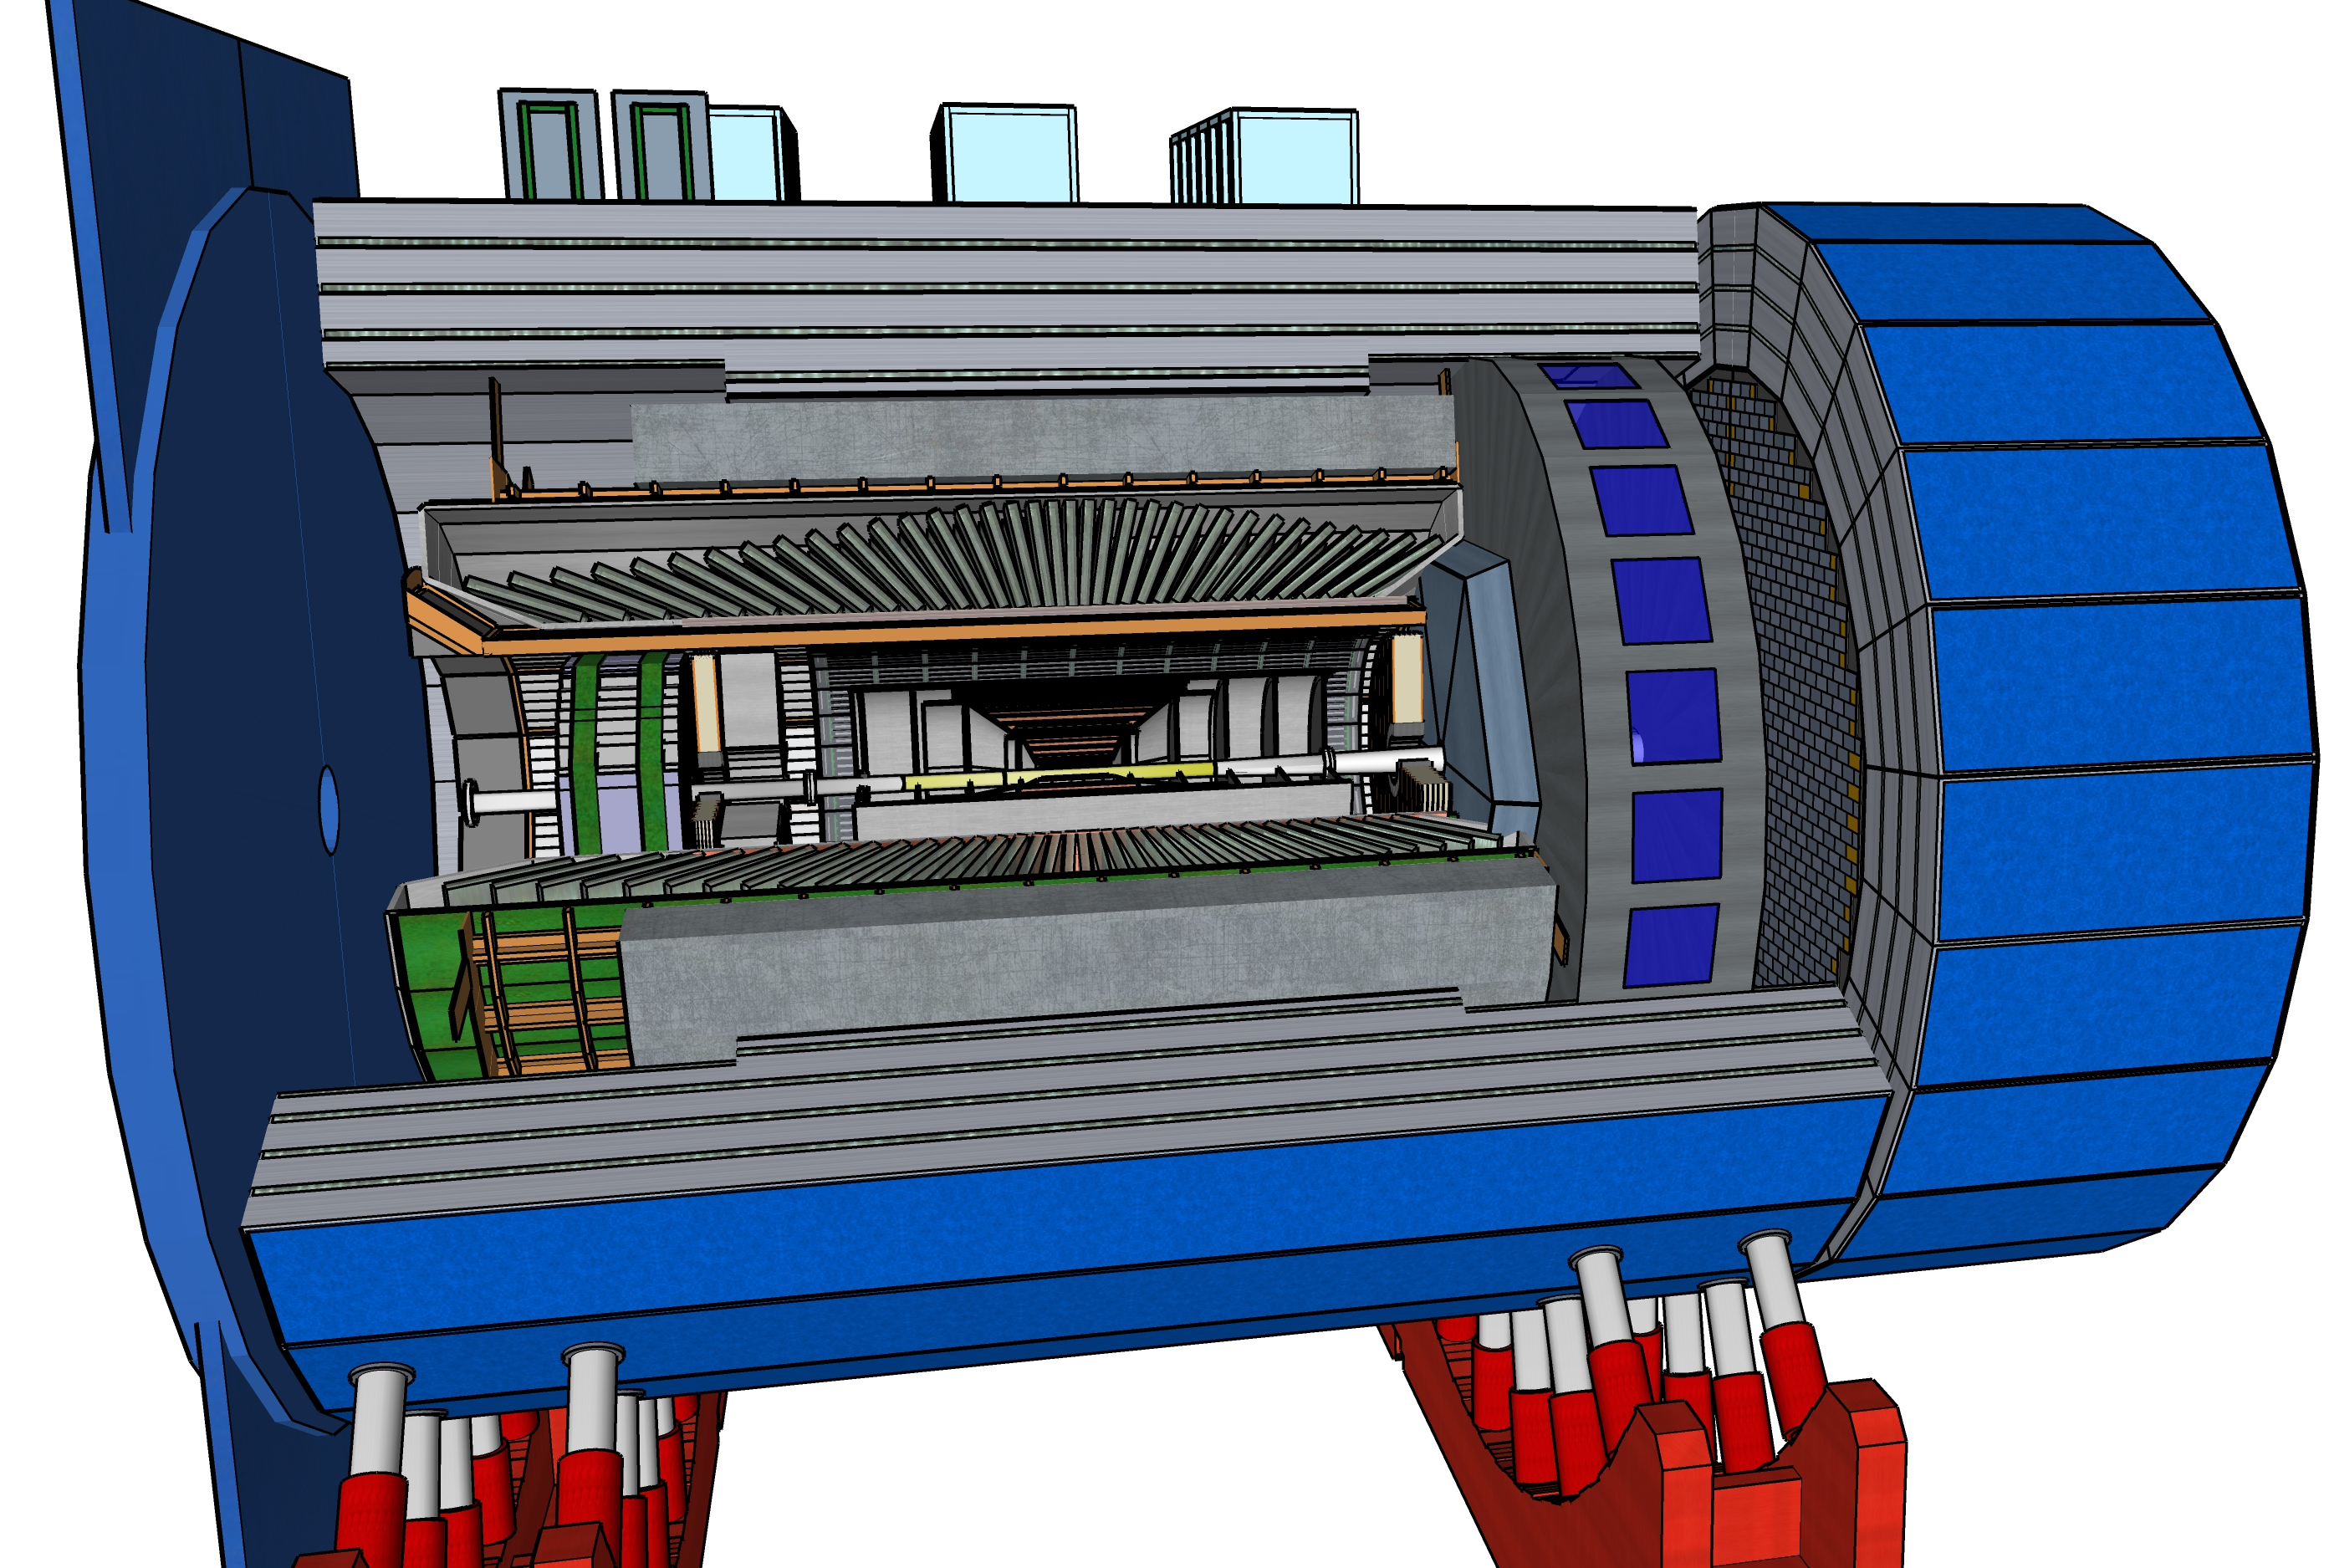
\includegraphics[width=0.7\linewidth]{figs/ECCE.png}
  \end{center}
\end{figure}
}


\vfill
\renewcommand*\familydefault{\rmdefault}


%\cleardoublepage
%\pagestyle{fancy}

\setcounter{page}{1}

%\clearpage
%\cleardoublepage

%\resetlinenumber

\tableofcontents
\clearpage

%\mainmatter

\renewcommand{\thepage}{\arabic{page}}
%\setcounter{chapter}{0}
%\setcounter{page}{1}

%%%%%%%%%%%%%%%%%%%%%%%%%%%%%%%%% 2 Detector Overview


\section {Overview}
\label{overview}
The purpose of this note is to document the plans by the ECCE consortium to re-use the BaBar solenoid.  The BaBar solenoid is currently planned for use in the sPHENIX experiment and will be available after sPHENIX running concludes in 2025. The solenoid provides a 1.4T central field at design current. 

The design parameters of the BaBar solenoid are shown in Figure~\ref{fig:BaBarStats}. 

\begin{figure}[h!tbp]
    \centering
    \includegraphics[width=0.9\textwidth]{figs/BaBar_Stats.png}
    \caption{Parmeters of the BaBar solenoid.}
    \label{fig:BaBarStats}
\end{figure}

\begin{figure}[h!tbp]
    \centering
    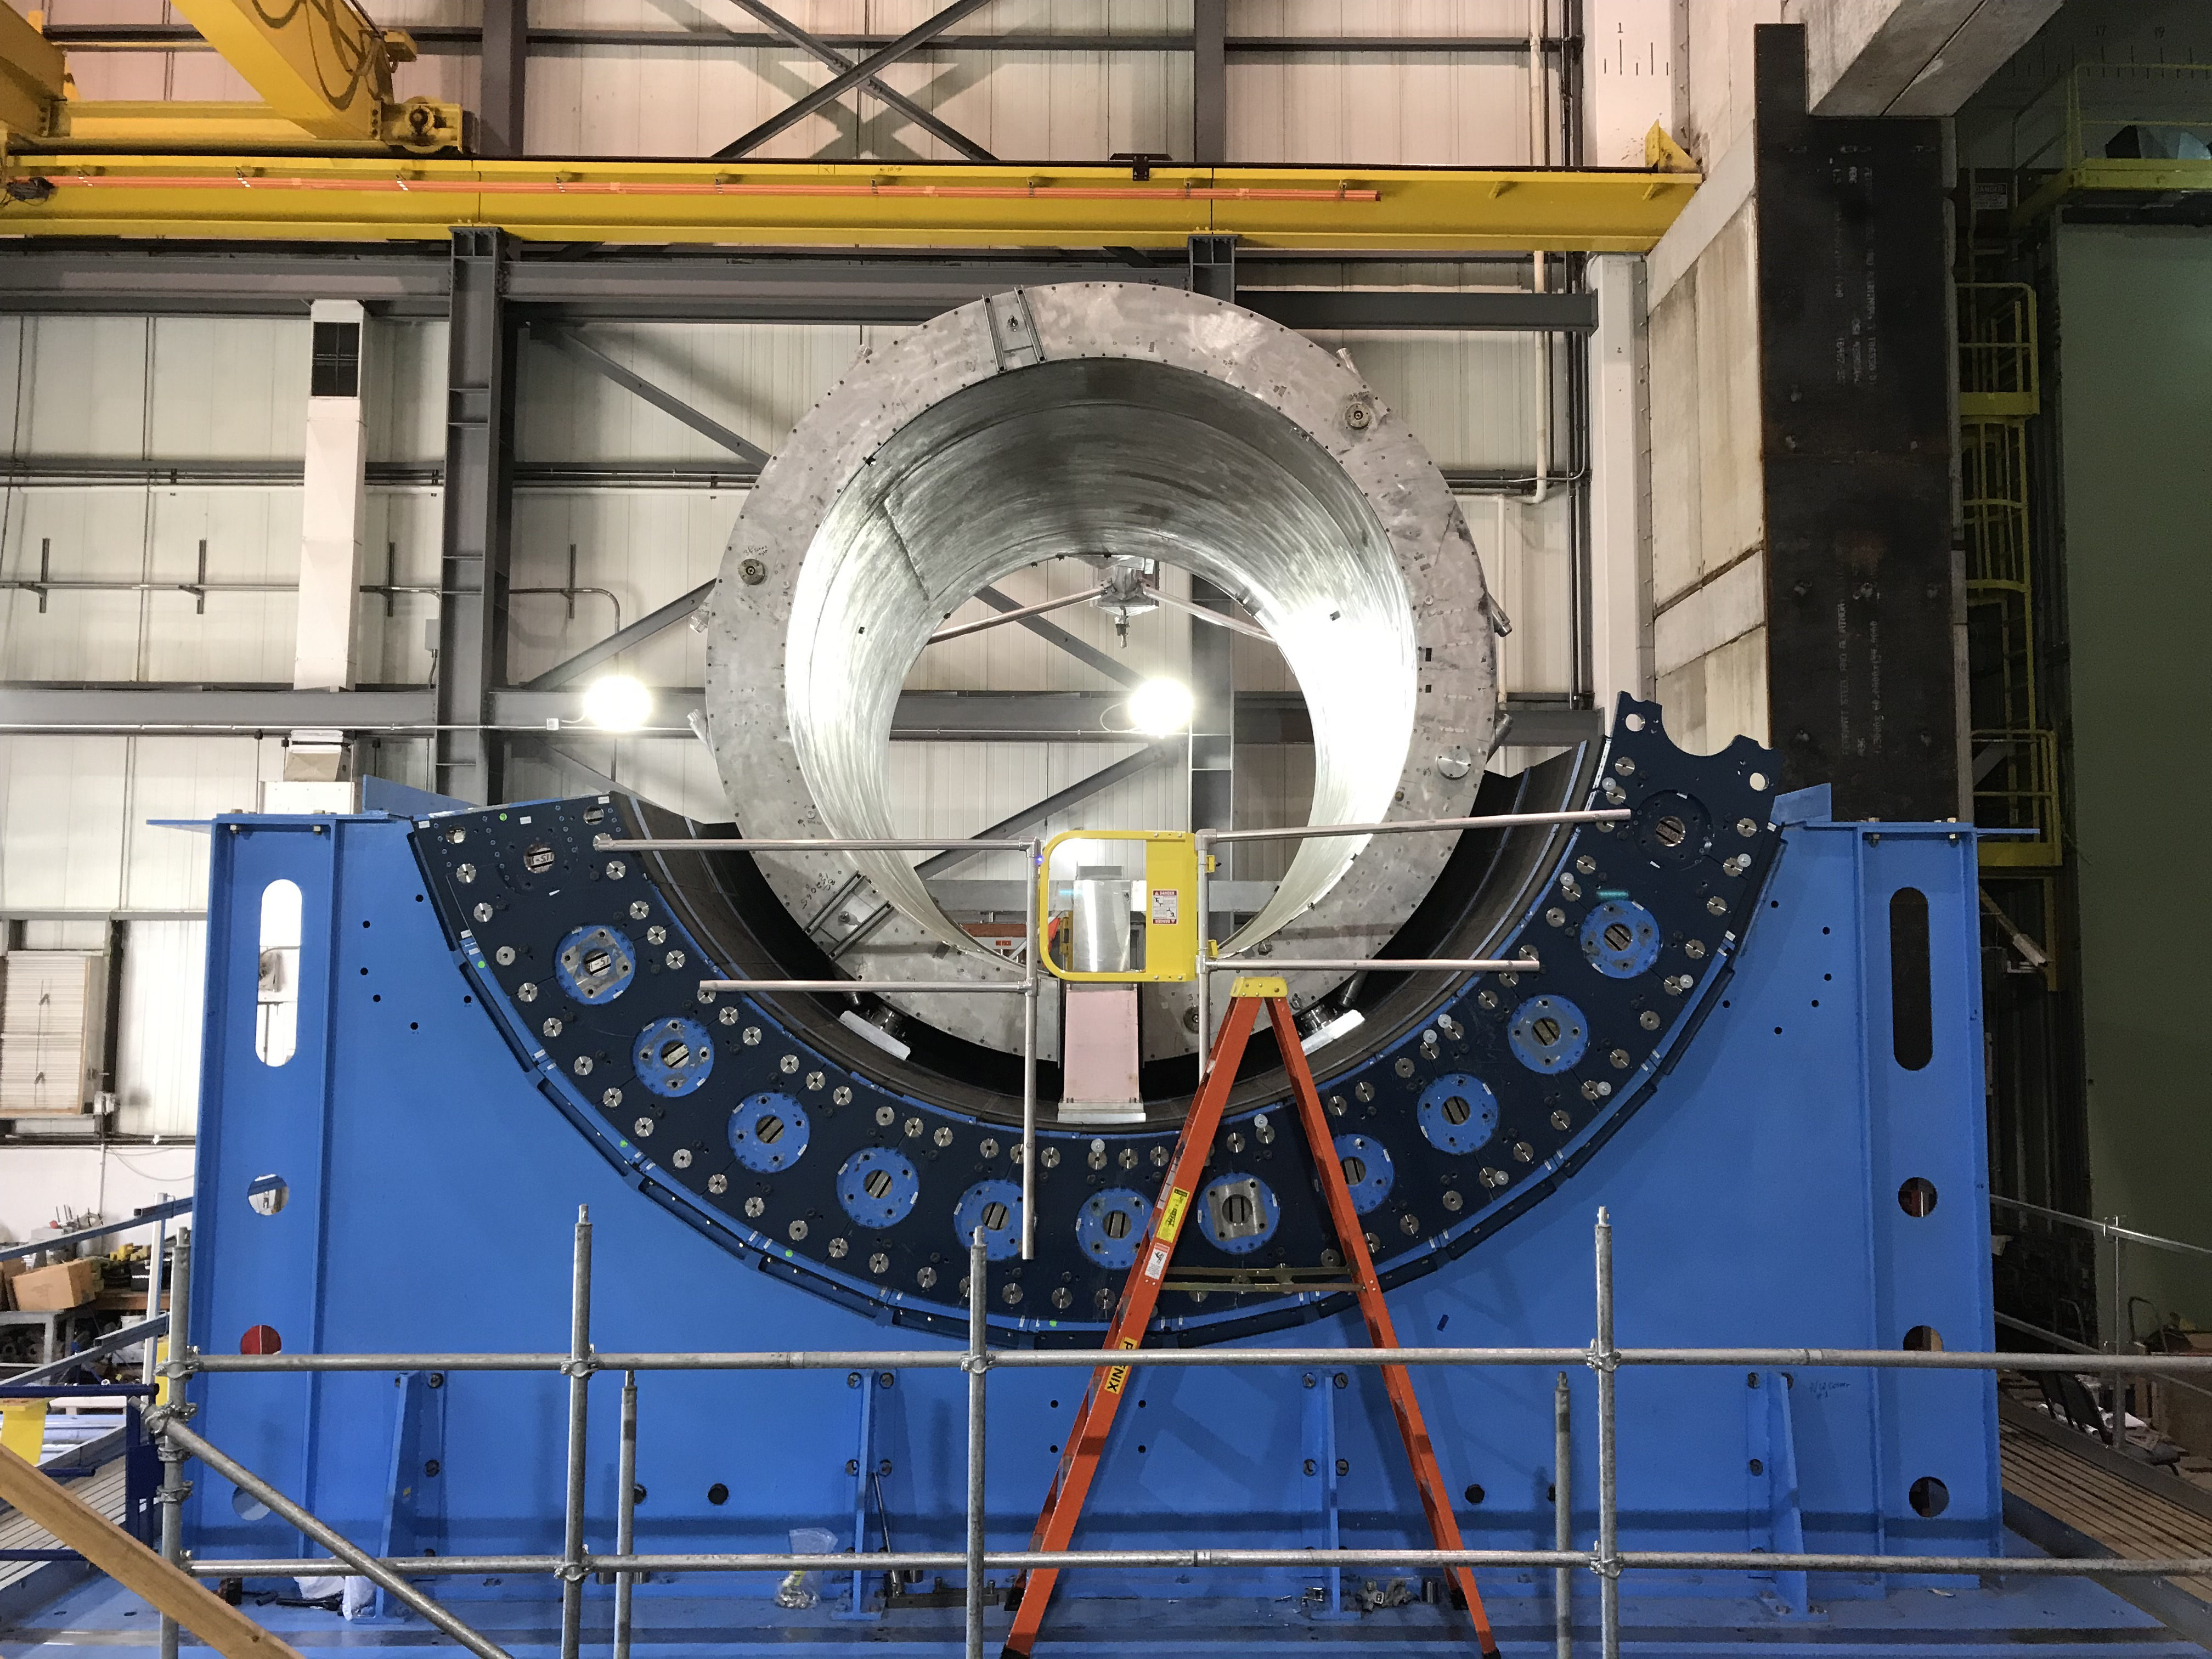
\includegraphics[width=0.9\textwidth]{figs/magnet_install_1.png}
    \caption{The BaBar solenoid in October, 2021, as it was installed in the sPHENIX experiment. The solenoid is resting in the barrel flux return, which will be completed with additional sectors in the coming months.  The experimental cradle, barrel flux return (outer hadronic calorimeter), and BaBar solenoid are all items planned to be re-used by the ECCE experiment.}
    \label{fig:BaBarInSPHENIX}
\end{figure}

\subsection{Refurbishment of the BaBar Solenoid}

The re-use of the magnet has been the subject of a engineering study and risk analysis, available as an EIC Technical Note (EICTJ-O-DE-PLT-TD-0017-R00), which also details the potential actions required to refurbish the BaBar solenoid for use in ECCE. 

After extensive discussions with the JLab engineers, it was decided that any modifications or refurbishment that required opening the BaBar solenoid cryostat would not be worth the additional risk. None of these actions will be necessary if the magnet continues to operate well throughout sPHENIX running. sPHENIX is expected to conduct a high-field magnet test in the experiment flux return (which will also be re-used for ECCE) in mid-2022, followed by experimental operations 2023-25. Figure~\ref{fig:BaBarInSPHENIX} shown the BaBar solenoid installed in the sPHENIX experiment. As a mitigation against the schedule risk posed by a problem with the BaBar solenoid developing late in sPHENIX running, we proceed with the initial engineering and design for a replacement magnet. It is expected a final decision to proceed with the BaBar solenoid or produce a new magnet will be taken in mid-2023 after the performance of the BaBar solenoid during the first year of sPHENIX running is reviewed by a panel of experts.  The risk-mitigation decision tree is shown in Figure~\ref{fig:risk_tree}. 

A draft schedule for the ECCE solenoid is shown in Figure~\ref{fig:magnet_schedule}. 

\begin{figure}[h!tbp]
    \centering
    \includegraphics[width=0.9\textwidth]{figs/flowchart_Page_1.png}
    \caption{Decision tree for the selection of either the ECCE magnet of a new magnet with the same characteristics.}
    \label{fig:risk_tree}
\end{figure}

\begin{sidewaysfigure}[h!tbp]
    \centering
    \includegraphics[width=1.0\textwidth]{figs/ECCE Detector Solenoid_Babar reuse_v5.png}
    \caption{Schedule for the ECCE solenoid.}
    \label{fig:magnet_schedule}
\end{sidewaysfigure} 
%The purpose of this note is to document the plans by the ECCE consortium to re-use the BaBar solenoid.  The BaBar solenoid is currently planned for use in the sPHENIX experiment and will be available after sPHENIX running concludes in 2025. The solenoid provides a 1.4T central field at design current. 

The design parameters of the BaBar solenoid are shown in Figure~\ref{fig:BaBarStats}. 

\begin{figure}[h!tbp]
    \centering
    \includegraphics[width=0.9\textwidth]{figs/BaBar_Stats.png}
    \caption{Parmeters of the BaBar solenoid.}
    \label{fig:BaBarStats}
\end{figure}

\begin{figure}[h!tbp]
    \centering
    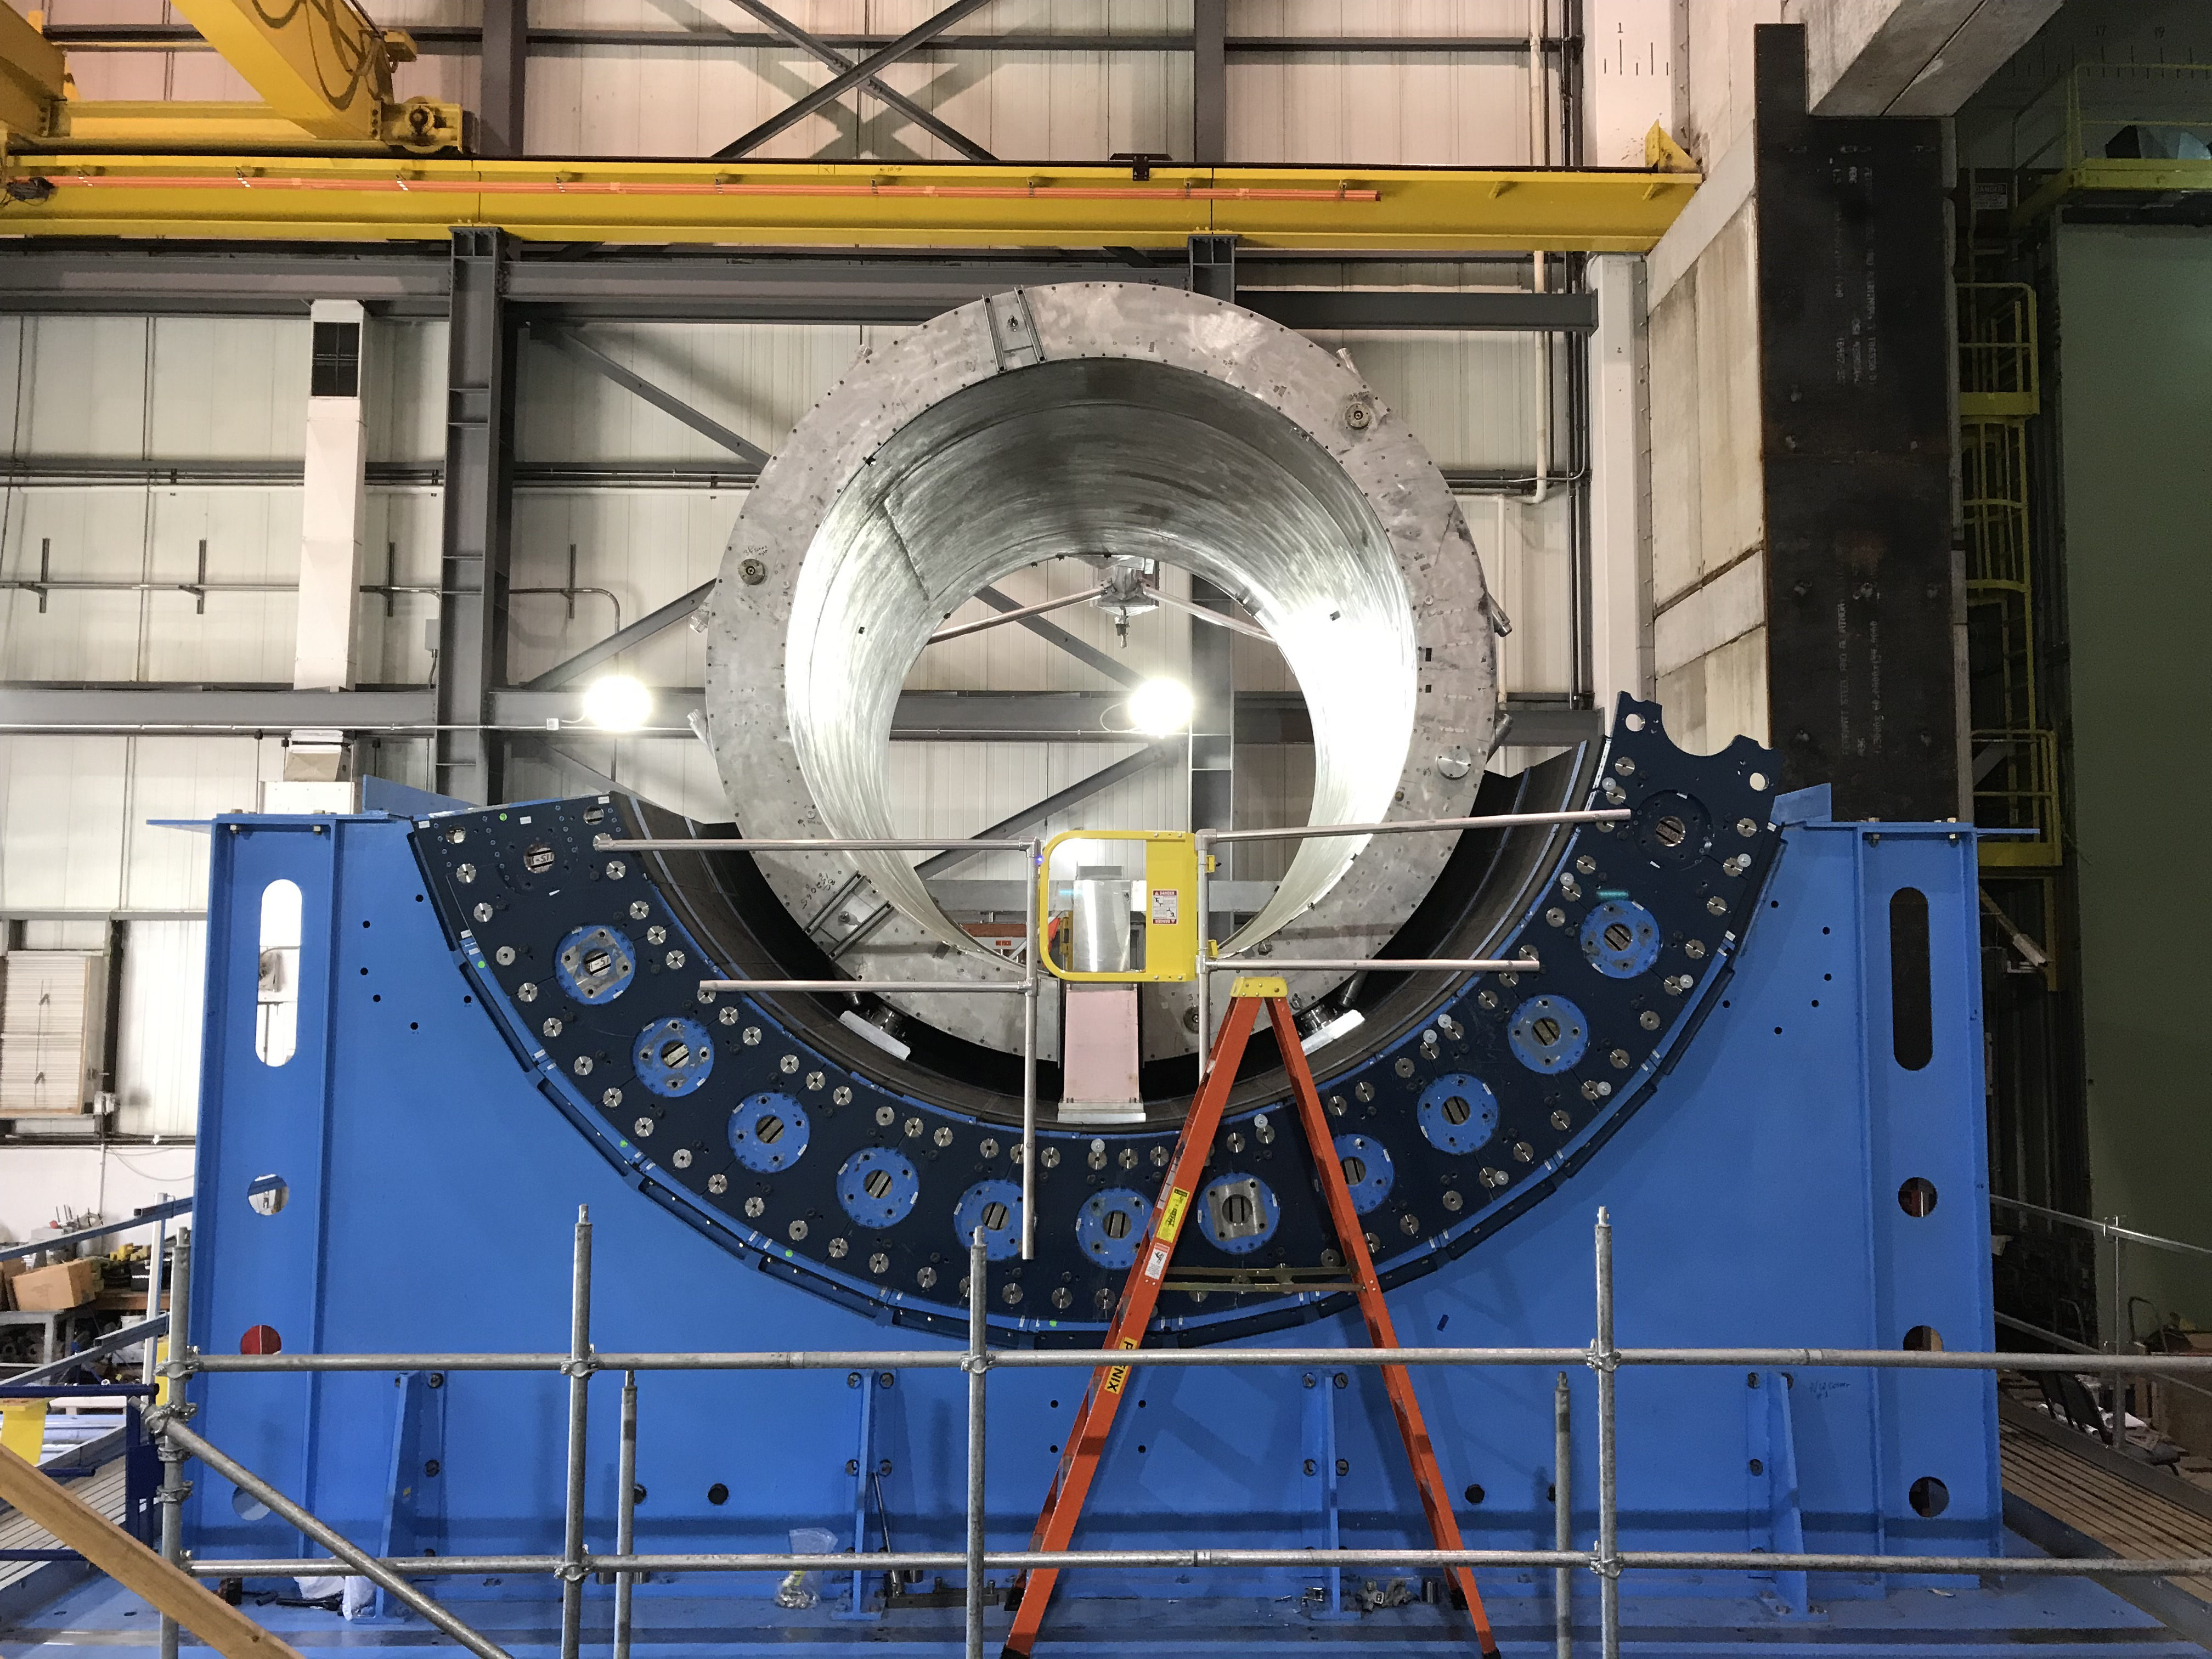
\includegraphics[width=0.9\textwidth]{figs/magnet_install_1.png}
    \caption{The BaBar solenoid in October, 2021, as it was installed in the sPHENIX experiment. The solenoid is resting in the barrel flux return, which will be completed with additional sectors in the coming months.  The experimental cradle, barrel flux return (outer hadronic calorimeter), and BaBar solenoid are all items planned to be re-used by the ECCE experiment.}
    \label{fig:BaBarInSPHENIX}
\end{figure}

\subsection{Refurbishment of the BaBar Solenoid}

The re-use of the magnet has been the subject of a engineering study and risk analysis, available as an EIC Technical Note (EICTJ-O-DE-PLT-TD-0017-R00), which also details the potential actions required to refurbish the BaBar solenoid for use in ECCE. 

After extensive discussions with the JLab engineers, it was decided that any modifications or refurbishment that required opening the BaBar solenoid cryostat would not be worth the additional risk. None of these actions will be necessary if the magnet continues to operate well throughout sPHENIX running. sPHENIX is expected to conduct a high-field magnet test in the experiment flux return (which will also be re-used for ECCE) in mid-2022, followed by experimental operations 2023-25. Figure~\ref{fig:BaBarInSPHENIX} shown the BaBar solenoid installed in the sPHENIX experiment. As a mitigation against the schedule risk posed by a problem with the BaBar solenoid developing late in sPHENIX running, we proceed with the initial engineering and design for a replacement magnet. It is expected a final decision to proceed with the BaBar solenoid or produce a new magnet will be taken in mid-2023 after the performance of the BaBar solenoid during the first year of sPHENIX running is reviewed by a panel of experts.  The risk-mitigation decision tree is shown in Figure~\ref{fig:risk_tree}. 

A draft schedule for the ECCE solenoid is shown in Figure~\ref{fig:magnet_schedule}. 

\begin{figure}[h!tbp]
    \centering
    \includegraphics[width=0.9\textwidth]{figs/flowchart_Page_1.png}
    \caption{Decision tree for the selection of either the ECCE magnet of a new magnet with the same characteristics.}
    \label{fig:risk_tree}
\end{figure}

\begin{sidewaysfigure}[h!tbp]
    \centering
    \includegraphics[width=1.0\textwidth]{figs/ECCE Detector Solenoid_Babar reuse_v5.png}
    \caption{Schedule for the ECCE solenoid.}
    \label{fig:magnet_schedule}
\end{sidewaysfigure}

\section {Estimated In-Kind Value}
\label{costing}
In this section we estimate the value of the BaBar solenoid as an in-kind contribution to the ECCE experiment, as well as the estimated cost to replace the solenoid if for some reason the BaBar solenoid is unavailable at the time of ECCE construction. 

\subsection{Magnet Cost Formulas}

A useful set of formulas for estimating the cost of a magnet as a function of the stored energy are available in the form of two papers, published in 1993 and 2008 \cite{Green1993,Green2008}. The estimated cost grows as a power of the stored energy and are given in 1993 and 2007 dollars, respectively. These formulas can be combined with the CPI inflation calculator (https://www.bls.gov/data/inflation\_calculator.htm) to arrive at an estimated value of the BaBar solenoid in 2021 dollars. Note that the 1993 paper formula calculates the values in 1993 dollars, while the 2008 paper formula is in 2007 dollars. 

The combined 1993 cost formula and inflation factor is: 

\begin{equation}
    C = 0.458 \times E(MJ)^{0.7} \times 1.91
\end{equation}

\noindent where $E(MJ)$ is the stored energy in MJ and the factor 1.91 is the inflation escalation to 2021 dollars. 

The same calculation using the 2008 formula yields: 

\begin{equation}
    C = 0.92 \times E(MJ)^{0.6} \times 1.34
    \label{eq:2008}
\end{equation}

With a stored energy of 27MJ, the estimated value in 2021 dollars of the BaBar solenoid using the 1993 formula is \$8.8M, while using the 2008 formula yields a value of \$8.9M. The two calculations are quite consistent with one another, yielding a value of the BaBar solenoid (to one significant figure) of \$9M. 


\subsection{Estimated Costs for Variations on the BaBar Solenoid}

The potential exists that the BaBar solenoid may not be available for use by ECCE at the time of ECCE construction, or that the cost of the refurbishment required may not be cost-effective. In this case it is possible that a new solenoid could be considered. Under these circumstances, the ECCE consortium could consider a higher magnetic field for the new solenoid. 
If we assume the same dimensions as the BaBar solenoid, the stored energy scales like the square of the magnetic field. While the BaBar solenoid is rated for 27MJ of stored energy, for a 2.0T solenoid of the same dimensions the stored energy would be 48MJ.  A 2.5T solenoid of the same energy would have a stored energy of 75MJ. 

Using the 2008 formula in Equation~\ref{eq:2008} and the stored energy calculated for the 2.0T and 2.5T field, the cost in 2021 dollars would \$12.6 and \$16.4M, respectively. The potential solenoid options are summarized in Table~\ref{tab:magoptions}. 

Note that a larger magnetic field will also imply additional engineering and design considerations, such as the differential force in the magnet coils due to the asymmetric nature of the ECCE flux return.  These are discused in Section~\ref{simulations}. 

\begin{table}[h!tbp]
    \centering
    \begin{tabular}{lcc}
        \hline
                     Magnet    & Stored Energy (MJ) &  Cost/Value (2021\$) \\ [0.5ex]
         \hline
%         BaBar Solenoid (1.4T) & 27 & 8.9M \\
         BaBar Solenoid (1.5T) & 27 & 8.9M \\       
         New Solenoid (2.0T)   & 48 & 12.6M \\
         New Solenoid (2.5T)   & 75 & 16.4 \\
         \hline
    \end{tabular}{}
     \caption{Tabular listing of the stored energy and cost for several ECCE solenoid options.}
    \label{tab:magoptions}
\end{table}




\section {Magnetic Field Simulations}
\label{simulations}
In this section we summarize the magnetic field simulations for use of the BaBar solenoid in ECCE.  These simulations were performed by Paul Brindza of Thomas Jefferson National Laboratory using the Opera computational tool. 

\subsection{ECCE Flux Return Configuration}

Simulations of the ECCE magnetic field configuration were done using OPERA (Tosca) for a central magnetic field of 1.5T, corresponding to a stored energy of $2.44\times 10^{7} J$.  Figure~\ref{fig:3DModel} shows the geometry of the 3D model for the OPERA calculations, while Figure~\ref{fig:BzOnAxis} shows the z component of the magnetic field along the central axis of the solenoid. 

\begin{figure}[h!tbp]
    \centering
    \includegraphics[width=0.9\textwidth]{figs/3DModel.png}
    \caption{Image of the 3D model used for magnetic field calculations within OPERA. Shown are the coil (red) and a cutaway of the flux return (blue). Note the asymmetric nature of the flux return on the forward going (right) side of the coil. }
    \label{fig:3DModel}
\end{figure}

\begin{figure}[h!tbp]
    \centering
    \includegraphics[width=0.9\textwidth]{figs/BzOnAxis.png}
    \caption{Magnetic field along the z-axis in the ECCE magnet.  Note that the coil is shifted in z with respect to the center of the coordinate system by +20cm. }
    \label{fig:BzOnAxis}
\end{figure}

\subsection{Estimated Forces on the BaBar Coils}

The asymmetric nature of the ECCE detector flux return will yield an asymmetric force on the BaBar solenoid coils. Forces on the magnet coils due to the asymetric arrangement were calculated within OPERA using the integral method (most accurate) and checked using hand calculations. Figure~\ref{fig:BRadial} shows the radial component of the magnetic field at the location of the solenoid coils. This component of the magnetic field will generate longitudinal stress on the coils. Figure~\ref{fig:BzThroughCoil} shows the z-component of the magnetic field at the location of the solenoid coils. This component of the magnetic field will generate a radial "hoop" stress on the coils. 

\begin{figure}[h!tbp]
    \centering
    \includegraphics[width=0.9\textwidth]{figs/BRadial.png}
    \caption{Radial component of the magnetic field at the coil location of $r=153cm$ along a line parallel to the z-axis from $z=-154cm$ to $z=194cm$.  }
    \label{fig:BRadial}
\end{figure}

\begin{figure}[h!tbp]
    \centering
    \includegraphics[width=0.9\textwidth]{figs/BzThroughCoil.png}
    \caption{Component of the magnetic field along the z-axis at the coil location of $r=153cm$ along a line parallel to the z-axis from $z=-154cm$ to $z=194cm$.  }
    \label{fig:BzThroughCoil}
\end{figure}

Table~\ref{tab:opera_forces} shows the force on each coil and the net force on the magnet calculated from OPERA using the integral method.  The unbalanced force on the magnet is 3600N (or 810lbs).  As a comparison, a hand calculation of the net forces on the coils is shown in Table~\ref{tab:hand_forces}, which yields a net force of 4211N (or 947 lbs).  It should be noted that the field differences that generate these forces are less than the model accuracy of 1.5\%. Overall, the unbalanced forces on the magnet are small because the magnetic field at the locations of the forward/backward calorimeters are small and most of the magnetic flux is returned through the barrel.  These small forces should not present a substantial engineering difficulty in the proposed ECCE configuration. 

\begin{table}
\centering
\begin{tabular}{c|c|c}
Coil & Location & Force (NT) \\
\hline
1 & center inner & 5988 \\
2 & center outer & 817 \\
3 & left(-) inner & 3,073,723 \\
4 & right(+) inner & -3,072,571 \\
5 & left(-) outer & 3,085,758 \\
6 & right(+) outer & 3,082,957 \\
\hline
Net Force & center inner & -3600 \\
Net Force (lbs) & center inner & 810 lbs \\
\end{tabular}
\caption{Coil forces calculated from field integrals in OPERA.}
\label{tab:opera_forces}
\end{table}

\begin{table}
\centering
\begin{tabular}{c|c|c|c}
Coils & Net $B_{avg}$ T & I (amps) & Force (NT) \\
\hline
1\&2 (center) & -0.00035 & -1484508 & +5022 \\
3\&5 (neg. side) & -0.39507 & -1709732 & +6,493,359 \\
1\&2 (pos. side) & +0.39563 & -1709711 & -6,502,592 \\
\hline
Total & $+1.47\times10^{-5}$ & -4903951 & -4211 \\
\end{tabular}
\caption{Net forces on coil pairs from a hand calculation using the average magnetic field using $F=B_{r}IL$, where $L=9.61m$.}
\label{tab:hand_forces}
\end{table}


\section {dRICH performance in magnetic field}
\label{dRICH}
Magnetic field modified the particle momentum, in particular $p_{x}$ and $p_{y}$, changing the entrance position and incidence angle to the dRICH. In this section we look at the impact of this effect over the dRICH performance. Figure~\ref{fig:drich_p4_xy} show Cherenkov ring produce by 4~GeV electrons, pions, and kaons with and without magnetic field. 
\begin{figure}[h!tbp]
    \centering
    \includegraphics[width=0.5\textwidth]{figs/rings_xy_p4_fornote.pdf}
    \caption{dRICH hits, from events including 4~GeV electrons, pions, and kaons.}
    \label{fig:drich_p4_xy}
\end{figure}
To understand the impact of the magnetic field we look at the modification of the radius and width of the ring of electrons, pions, and kaons for three values of momentum, 1, 4, and 10~GeV. Figure~\ref{fig:drich_pX_e} shown dRICH hits centered at (0,0) in $(\eta,\phi)$ space with and without the magnetic field. We can see for 1~GeV electrons there is small smear of the inner (Gas) ring when the magnetic field is turned-on. 
\begin{figure}[h!tbp]
    \centering
    \includegraphics[width=0.9\textwidth]{figs/rings_etaphi_electron.pdf}
    \caption{dRICH hits for 1, 4 and 10~GeV electron events.}
    \label{fig:drich_pX_e}
\end{figure}
The radius distribution is calculated as $R=\sqrt{\phi^{2}+\eta^{2}}$ for each dRICH hit, we can compare this with magnetic field turned-on and off. In Figure~\ref{fig:drich_radius_p1_ePiK} we can see a small tail in the radius distribution for Gas ring of low p electrons. This small modification in the radius width is not expected to cause a degradation in the PID performance.
\begin{figure}[h!tbp]
    \centering
    \includegraphics[width=0.7\textwidth]{figs/Radius_p1_shift.pdf}
    \caption{Radius distribution of 1~GeV electrons, pion and kaons.}
    \label{fig:drich_radius_p1_ePiK}
\end{figure}

\listoftodos[To Do]

\bibliographystyle{unsrturl}
\bibliography{refs}

\end{document}  
%%%%%%%%%%%%%%%%% End Document
